\section{Background}

XAI is the interpretation and explanation of machine learning models.  In order to go further, the concepts of "interpretation" and "explanation" warrant a more formal definition:

\begin{itemize}
    \item an \textbf{interpretation} is the mapping of an abstract concept (e.g. a predicted class) into a domain that the human can make sense of, and
    \item an \textbf{explanation} is the collection of features of the interpretable domain, that have contributed for a given example to produce a decision (e.g. classification or regression) \cite{MONTAVON20181}.
\end{itemize}

Sample human-interpretable domains include visual aids, natural language, or a more easily interpretable model, such as a decision tree.  An explanation is the relationship between a human-interpretable concept, such as words, images, or logic, and a query of how or why a machine learning model made a decision.  There is ambiguity and a lack of formality around the concept of an interpretation that is discussed further in \ref{sec:Challenges} \textit{Challenges in XAI}.

Some trained ML models may have easier-to-explain internals than others.  Decision trees are a common example of an explainable ML model.  The output of the decision tree can be directly traced back to identify the values of specific features that lead the model to its decision.  On the other hand, the internals of DNNs, by default, are opaque and are not directly interpretable.  Any node in the output layer of a neural network has many inputs with many weights, each of which may have many more inputs with many weights.  The value of a single input feature can propagate through virtually every node in a neural network, making it challenging to isolate the contribution of the value of a single feature in the output of the model.  In addition to the challenge in tracing a single feature through the a DNN, a single feature, such as the pixel in an image, may not have an isolated interpretation for humans to understand.  In that sense, the relevancy of an isolated input feature may not have meaning or value from a human's perspective.  Other difficult-to-explain machine learning models include support vector machines (SVM), random forests, and Gaussian belief networks (see figure \ref{fig:gunning2016}).

\begin{figure*}
    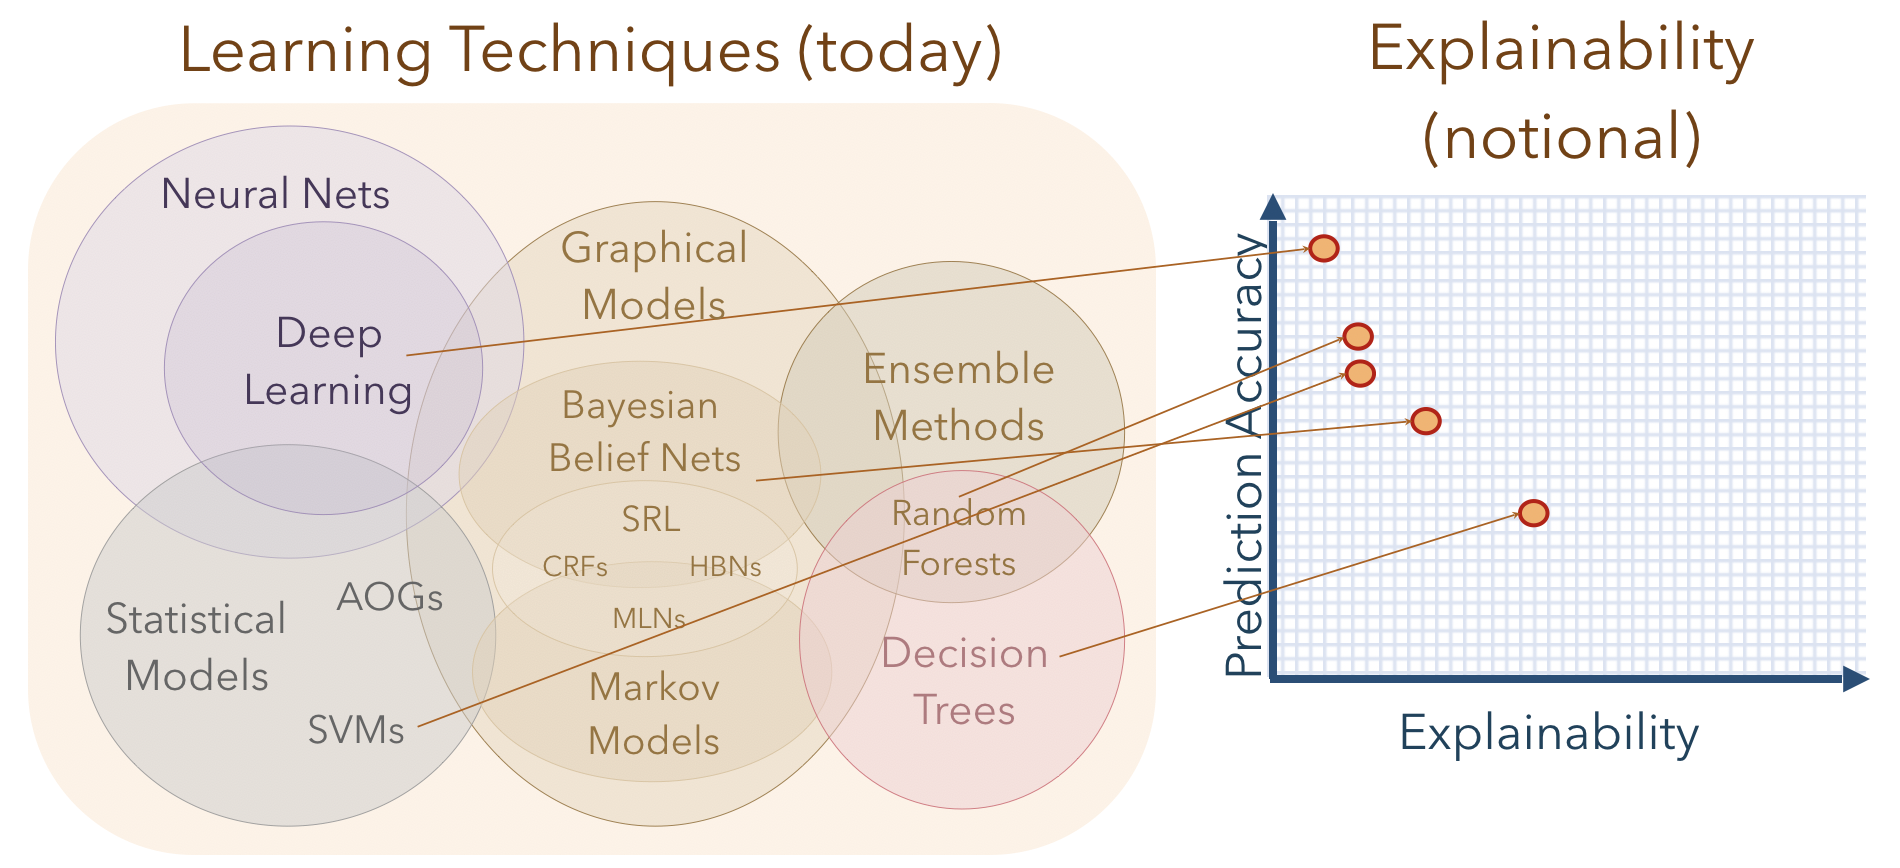
\includegraphics[width=\textwidth]{media/gunning2016.png}
    \caption{A visual comparison of the explainability of machine learning methods and their relative performance \cite{GunningXAI}.}.
    \label{fig:gunning2016}
\end{figure*}

There are various methods of XAI that can be applied in machine learning, both during or after the training of the ML model.  \textit{A priori} methods are those in which a traditionally black box model can be constructed in such a way that it either is easier to explain with other methods or can generate an explanation alongside its traditional output.  Examples of generated explanations include using a LSTM DNN alongside a CNN to generate natural language explanations \cite{10.1007/978-3-319-46493-0_1} or embedding prototypes of outputs classes directly in the CNN \cite{Chen2018}.  \textit{A posteriori} methods of XAI include visualizations techniques such as Deep Taylor decomposition and Layer-wise Relevance Propagation to generate heat maps that can be over-layed on the original input to help identify patterns in the relevancy of input features, such as highlighting outlines, regions, or other patterns that either supported or detracted from the network's decision.

In this section, methods of XAI or organized into the types of artifacts that are generated: visualization, verbalization, data provenance, and model induction.

\subsection{Visualization Techniques}

\subsubsection{LRP}

Layer-wise relevance propagation (LRP) is an \textit{a posteriori} method of generating heat maps, or saliency maps, to highlight the positive and, sometimes, negative relevancy of input features in the output layer, or decision, of a DNN \cite{MONTAVON20181}.  LRP is functionally a backward pass of the output layer back through the neural network to the input layer.  At its core, LRP is not a mathematical function but a set of constraints that defines properties of the relationship between layers in a DNN.  Data scientists can substitute existing or new activation functions to apply different highlight with different levels of sensitivity the relationship between the input and output layers of the DNN.

The heat maps generated by LRP are not limited to image inputs.  Researchers have applied heat maps generate dy LRP to natural language, genetic sequences, and 3D models of molecules (see figure \ref{fig:montavan2018}).

\begin{figure}
    \centering
    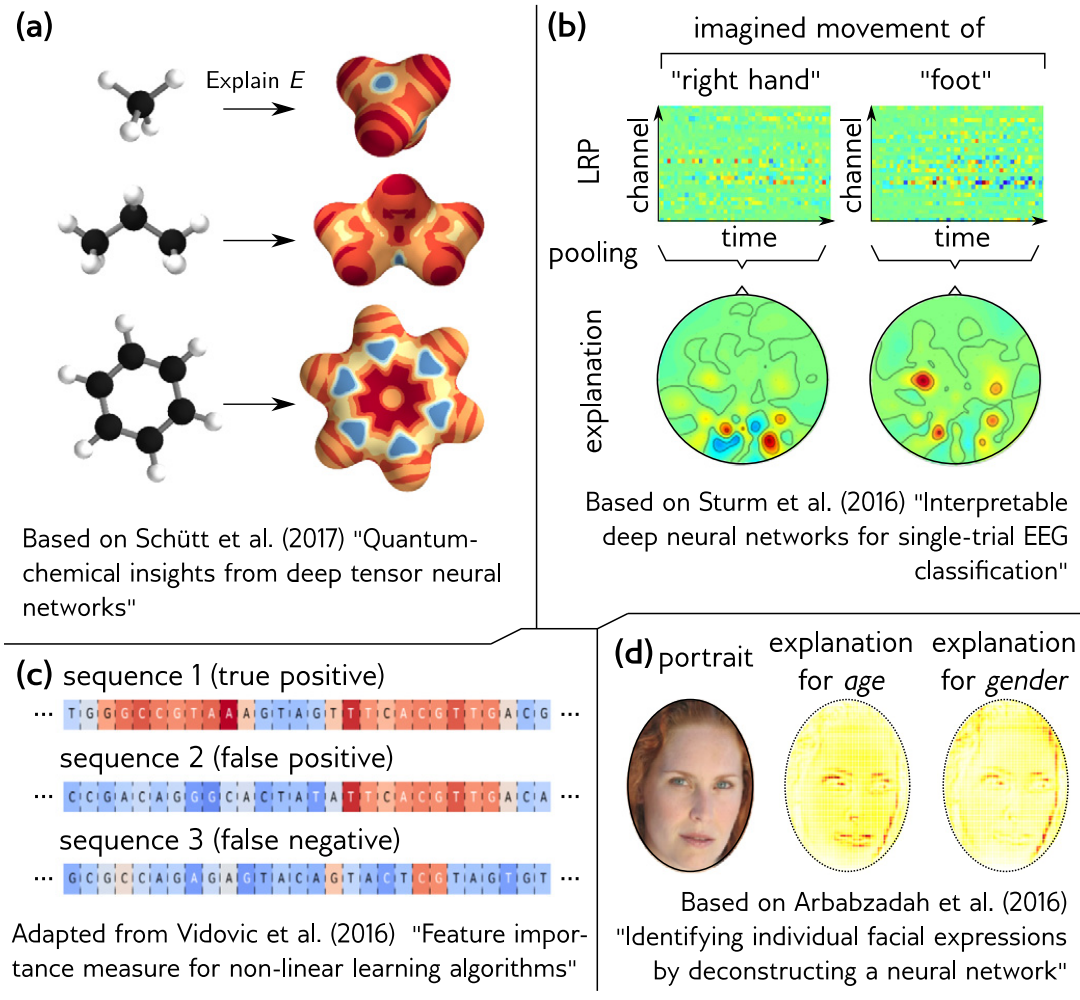
\includegraphics[width=3.4in]{media/montavan2018.png}
    \caption{Overview of several applications of machine learning explanation techniques in the sciences. (a) Molecular response maps for quantum chemistry, (b) EEG heatmaps for neuroimaging, (c) extracting relevant information from gene sequences, (d) analysis of facial appearance. \cite{MONTAVON20181}.}
    \label{fig:montavan2018}
\end{figure}

\subsubsection{Activation maximization}

Activation maximization is an \textit{a posteriori} method for generating an input for a model that maximizes the activation of a specific output neuron\cite{Nguyen2016}, such as a class label.  In theory, the input that maximizes the output would be some sort of ideal or target input, but in practice, the input that maximizes the activation of a neuron in the output layer may not lack human interpretability.  As seen in figure \ref{fig:nguyen2016}, the effectiveness of AM is largely network-specific.  However, the ideal input for a neural network may grant insights into what types of features a DNN favors for an output neuron.

\begin{figure*}
    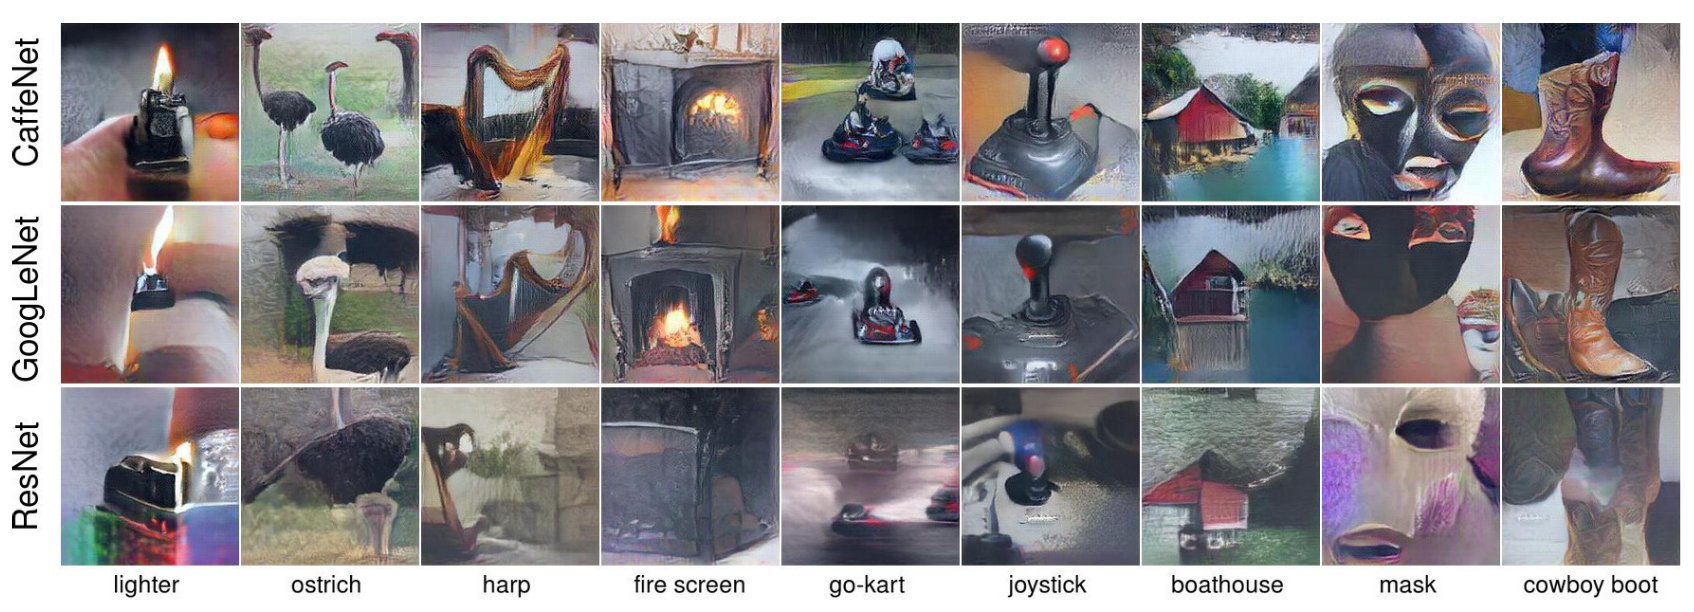
\includegraphics[width=\textwidth]{media/nguyen2016.png}
    \caption{Ideal inputs of various output classes for three different CNNs \cite{Nguyen2016}.}
    \label{fig:nguyen2016}
\end{figure*}

\subsubsection{Prototypes in CNNs}

Thus far in research, the concept of building a CNN with an \textit{a priori} prototype layer has been applied in image classification tasks \cite{Chen2018}.  A prototype is essentially an image or subset of an image of one of the target labels of the classifier, either from the training data or from an image of the target class from outside of the training data.  Each prototype could target a characteristic of the target class that has high relevance for human experts, such as a specific color pattern on a bird or an architectural feature of a building.  The class prototypes are used to construct a "prototype layer" between the convolutional layers and max pooling layer of a CNN.  When the prototype layer is constructed from subsets of training images, the theory is that each prototype represents some interpretable, defining characteristic of the class, such as a color pattern on a bird or the shape of ears on a bear.  Once a CNN has been constructed using a prototype layer, a data scientist can inspect the activation of various prototypes from that layer to gain insights into the importance of those characteristics in the CNN's decision.

\subsection{Verbalization of Explanations}

\subsubsection{Generating explanation in parallel}

CNNs excel at tasks of image classification, and long short-term memory (LSTM) networks excel with processing natural language, but their features can be combined \textit{a priori} such that an LSTM can be used to generate an explanation of why a CNN made its decision \cite{10.1007/978-3-319-46493-0_1}.  Such a hybrid model is trained jointly with labeled images and textual, natural language descriptions of those images.  Features of an input image are extracted from the convolutional layers of a CNN and supplied as input to an LSTM that has been trained to generate natural language responses based on the training descriptions (see figure \ref{fig:hendricks2016})

\begin{figure*}
    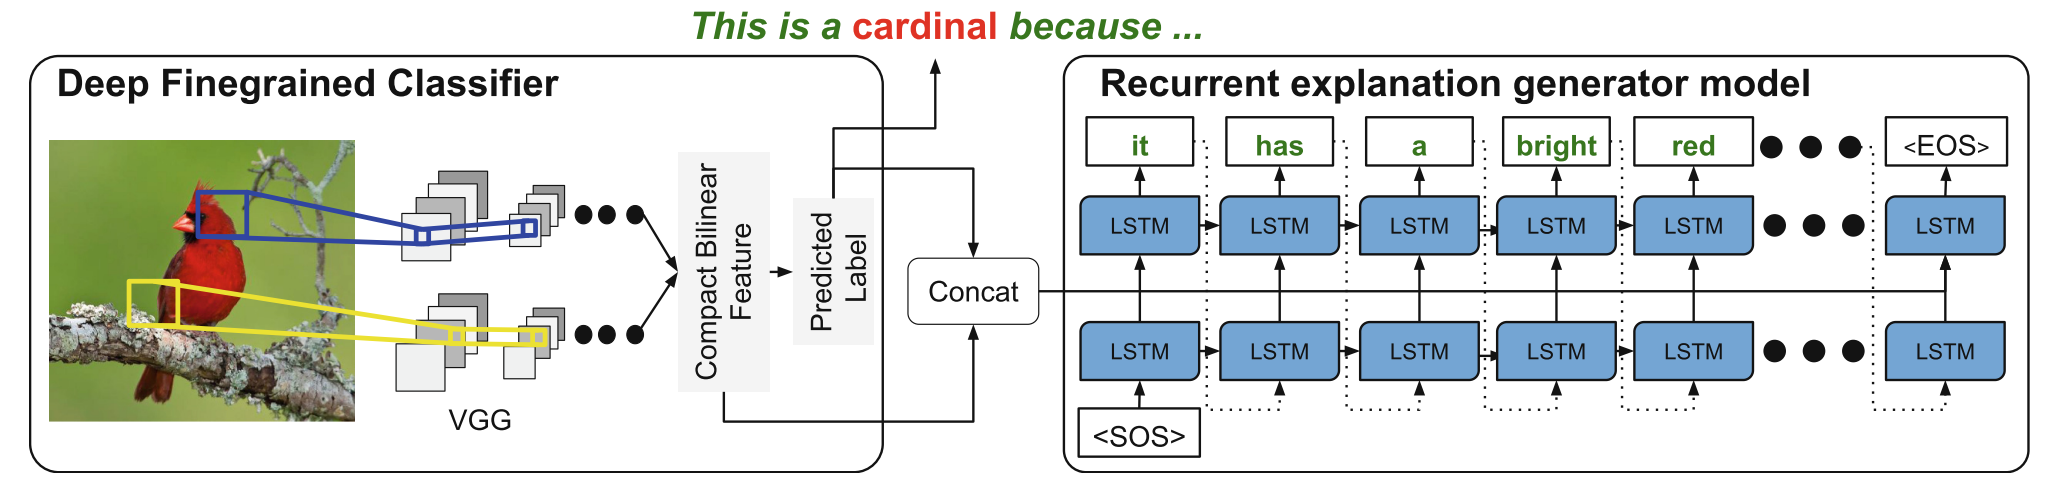
\includegraphics[width=\textwidth]{media/hendricks2016.png}
    \caption{Hybrid network architecture for generating classification decisions and accompanying textual descriptions of key features \cite{10.1007/978-3-319-46493-0_1}.}
    \label{fig:hendricks2016}
\end{figure*}

\subsubsection{Counterfactual explanations}

Counterfactual explanations are an \textit{a posteriori} method for generating bounds and rules for a classifier's decision.  For example, “you were denied a loan because your annual income was £30,000. If your income had been £45,000, you would have been offered a loan" \cite{DBLP:journals/corr/abs-1711-00399}.  Counterfactual bounds are extracted by algorithms that generate slight perturbations in an input's features until an observable change is made in the classifier's decision \cite{DBLP:journals/corr/abs-1711-00399}.  While the perturbation of input features may be compute intensive, the generation of counterfactual explanations requires no \textit{a priori} knowledge of the model's internals and circumvents the need to apply model- or topology-specific methods.  Counterfactual explanations work best when the input features are already human-interpretable as independent features, like income in the example above.  Counterfactual explanations generated from the perturbation of individual pixels in an image may not result in human-interpretable changes in the image \cite{DBLP:journals/corr/abs-1711-00399}.

\subsection{Data Provenance}

While other methods of XAI mostly focus on interpreting or explaining a model's decision based on evaluating new input, data provenance can explain how a model was created or how the training data relates to a decision.  Applying the principles of data provenance to the development of ML models establishes transparent data lineage throughout the life cycle of the data.  Being able to trace the history of the data provides benefit particularly for data scientists and auditors of ML systems.  Data scientists can develop ML models more collaboratively when they are able to log and share the various steps that have been applied in their workflows and their results, and auditors may analyze the history of the data to help identify potential issues with bias or discrimination.  If an opportunity to reduce bias or discrimination is discovered, then having a healthy lineage of the data should help data scientists in reducing effort in training a new model by exercising lessons learned and observations from previous development.

The taxonomy of concepts of data provenance may be high-level or even vague at times, but the core concepts lend themselves well to practical usage, such as the modeling, capturing, and persisting metadata \cite{Simmhan:2005:SDP:1084805.1084812}.  There exist many tools for generic data provenance activities, like managing the overhead and the scaling of metadata capture \cite{Simmhan2005ASO} or capturing data lineage by wrapping ETL pipelines \cite{Interlandi2017}; however, there are also software tools that are establishing themselves as ML-centric by integrating directly with existing ML libraries or offering their own libraries for common ML activity.  MLflow is a python library that provides metadata logging and collaboration features by integrating with common ML libraries, including Tensorflow, scikit-learn, Spark ML, and PyTorch \cite{Zaharia2018}.  H20.ai is a platform that focuses more inter-language operability by providing python, scala, R, and java APIs for their data provenance platform which includes libraries for feature extraction, dimension reduction, classification, and other common activities for training models \cite{H20.ai}.  Software tools and libraries for machine learning are becoming more accessible to wider audiences of data scientists, and there is industry demand for data provenance solutions that support heterogeneous machine learning platforms \cite{Schelter2017}.

\subsection{Model Induction}

Similar to counterfactual explanations, rules can be extracted from a black-box model by submitting a very large number of inputs whose input features vary only slightly from one to the next.  As bounds on the input features are discovered, these bounds result in rules which can be converted into an interpretable model, such as a decision tree of arbitrarily-constrained size.  Over a large enough data set, a set of rules may be an adequate approximation of the black-box model, often performing better than if a decision tree was trained directly from the data set \cite{Vandewiele2016GENESIMGE}.  Again, similar to counterfactual explanations, model induction works best when the input features are interpretable as independent of each other so that extracted rules may be more intuitive.  However, it remains possible to apply model induction to image inputs.  Frosst et al. extracted a decision tree from a neural network that was trained to play the game Connect Four \cite{Frosst2017DistillingAN} and observed that the first two layers of the decision tree may split the game the game into two routes: placement of pieces gravitate towards the center of the board or placement of pieces is more even distributed across all columns of the board \cite{Frosst2017DistillingAN}.  As seen in figure \ref{fig:frosst2017}, the interpretation of the decision tree is still highly subjective for visual inputs and relies on the observer's intuition.

\begin{figure}
    \centering
    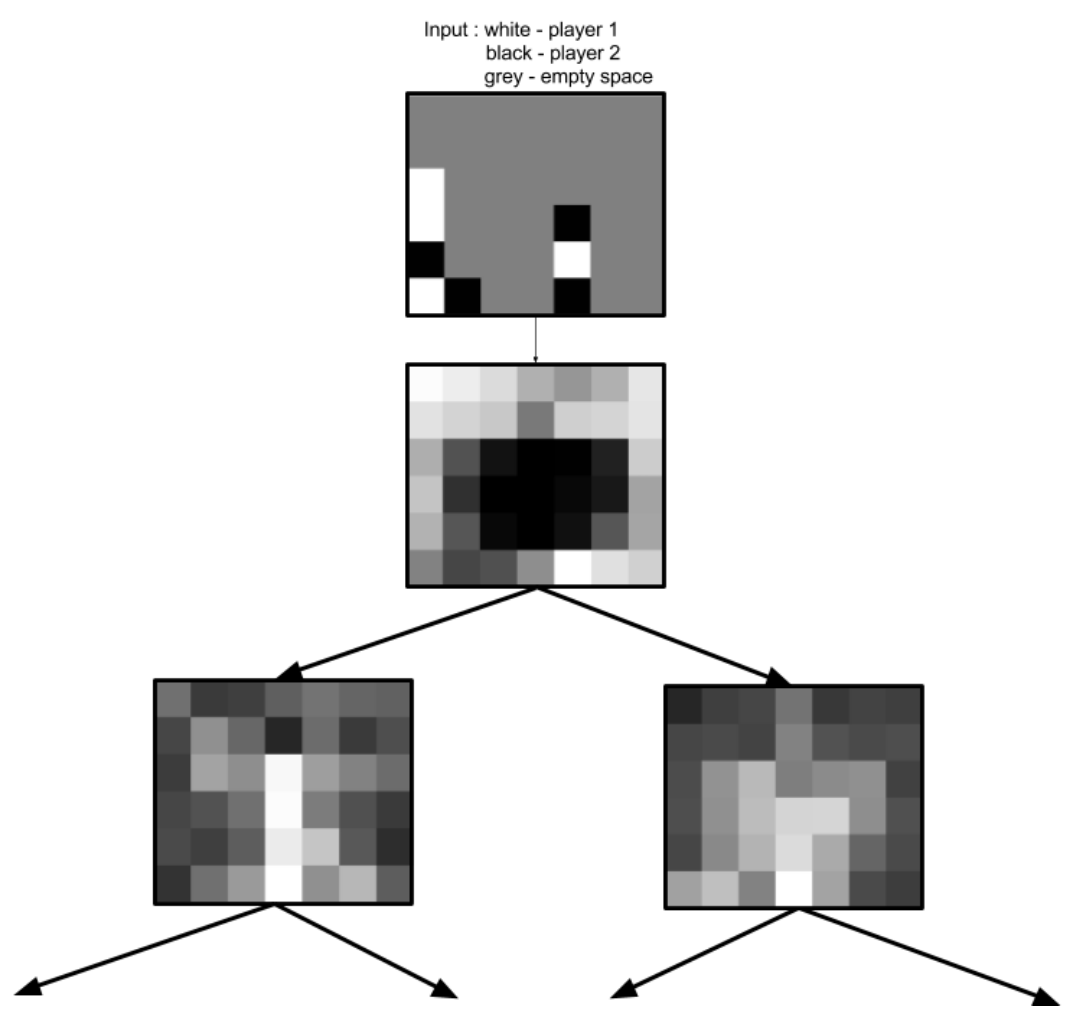
\includegraphics[width=3.4in]{media/frosst2017.png}
    \caption{The first two layers of a decision tree model extracted from a neural network that was trained to place pieces in the game of Connect Four \cite{Frosst2017DistillingAN}.}
    \label{fig:frosst2017}
\end{figure}

\subsection{Existing Surveys in XAI}

Although XAI is a relatively young field of research, appearing in publications circa 2016, there are at least hundreds of publications on the topic along with accompanying literature surveys that draw from the breadth of research.  Surveys vary in their perspective of XAI, the methods used to categorize literature, and the scope of methods that they cover.

Hohman et al. conduct a thorough literature search of visualization techniques of XAI \cite{Hohman2018}.  The authors' perspective begins with an analysis of the taxonomy of questions that can be asked of machine learning models.  The visualization techniques are labeled with various helpful metadata, such as what type of visualization is produced, if the XAI method is \textit{a priori} or \textit{a posteriori}, and more.  This metadata on the visualization techniques allows the reader to easily map the various visualization techniques to the questions that they can answer.

Montavon et al. present a far more focused literature search on a specific method of visualization in XAI and how it has been applied by other researchers, which domains, and to what ends \cite{MONTAVON20181}.  For a large portion of the paper, the method of Layer-wise Relevance Propagation (LRP) is broken down into its core mathematical principles so and trace those principles through a conceptual CNN to demonstrate how LRP may be applied to generate heat maps of input features to understand feature relevancy.  The authors to provide examples of LRP being applied in domains such as computer vision, genetic engineering, and chemistry.

The approach of Abdul et al. is to plot the relationship of topics around the interpretation and explanation of machine learning through the use of network graph visualizations \cite{Abdul:2018:TTE:3173574.3174156}.  This contribution to the surveying of XAI literature provides a much needed compass since the terminology in XAI, and even the name of the field itself, is still evolving rapidly.  We can also observe the relationship of topics in XAI as they weave through such domains as psychology, human-computer interaction, and the sociological aspects of accountability and fairness.

Guidotti et al. take a more broad approach to XAI methods by analyzing to what type of ML models have researchers been applying explanation methods, what were the interpretable domains of their inputs (e.g. images, natural language), and what methods of explanation were applied \cite{Guidotti:2018:SME:3271482.3236009}.  In this survey, a unique amount of attention was paid to methods of rule or model extraction, in which data scientists can extract a decision tree model or natural language rules as approximations of the original ML model.

Adadi et al. also take look at the methods of XAI as a whole and describe considerable detail on the non-visualization methods of XAI \cite{Adadi2018}.  In addition to their discussion on the taxonomy of XAI methods, this survey tracks the history of the terminology around XAI, exposing the burgeoning growth of the field and providing insight on the demands being placed on the field.  The authors classify the value provided by XAI into four different areas: explain to justify, explain to control, explain to improve, and explain to discover.

In some sense, the abundance of literature in such a short period of time speaks to the demand for further research in the field and to the wide-held interest across people of many backgrounds.  Time will tell if XAI can deliver the value that people seek or, perhaps, if societal impressions of AI/ML will evolve to no longer be concerned with the inner workings of machine learning.
